\section{Normalization} \label{sec:Normalization}

The vectors $\mathbf{x}_i$ of matrix $\mathbf{X}$ were normalized with the L1-norm to align the k-mer frequency vectors located in the rows to an equal length of one (\autoref{fig:Vectorization_Pipeline} \textsf{\textbf{B}}) (\autoref{eq:l1_norm} to \autoref{eq:l1_result}). The \textbf{preprocessing.normalize} function from the \textbf{scikit-learn (sklearn)} package, with \colorbox{backcolour}{norm='l1'} setting was used for the normalization \autocite{pedregosa_scikit-learn_2011}.

%\begin{lstlisting}[language=python]
%sklearn.preprocessing.normalize(M, norm='l1')
%\end{lstlisting}  

\begin{empheq}{alignat = -1}
    \mathbf{\hat{x}}_i &= \frac{\mathbf{x}_i}{\Vert\mathbf{x}_i\Vert_1} \label{eq:l1_norm}
\end{empheq}

\begin{empheq}{alignat = -1}
    \Vert\mathbf{\hat{x}}_i\Vert_1 &= 1\label{eq:l1_result}
\end{empheq}

The parameters used in this project with settings varying from the default are listed below. All available settings can be fount in the \href{https://scikit-learn.org/stable/modules/generated/sklearn.preprocessing.normalize.html}{API} \autocite{pedregosa_scikit-learn_2011}.

\begin{leftbar}
    \textbf{sklearn.preprocessing.normalize}
    \begin{nstabbing}
        \qquad\qquad\qquad\qquad\qquad\quad\=\kill
        
        X \> [Input matrix to be normalized]\\
        
        norm \> [Norm used for normalization (default: ’l2’)]
        
    \end{nstabbing}
\end{leftbar}

Due to an open\footnote{last accessed 02/06/21} \href{https://github.com/scikit-learn-contrib/hdbscan/issues/69}{issue} in the GitHub Repository of \gls{HDBSCAN} row-wise normalization with \textbf{preprocessing.normalize} was again used with the \colorbox{backcolour}{norm='l2'} setting, right before clustering. (\autoref{eq:l2_norm} to \autoref{eq:l2_result} and \autoref{fig:Clustering_Pipeline} \textsf{\textbf{D}}). It was stated, normalization with L2-norm prior to clustering with euclidean metric setting, chord distance, which is also not directly available, can be used to approximate cosine distance.

\begin{figure}[!hbt]
    \centering
    %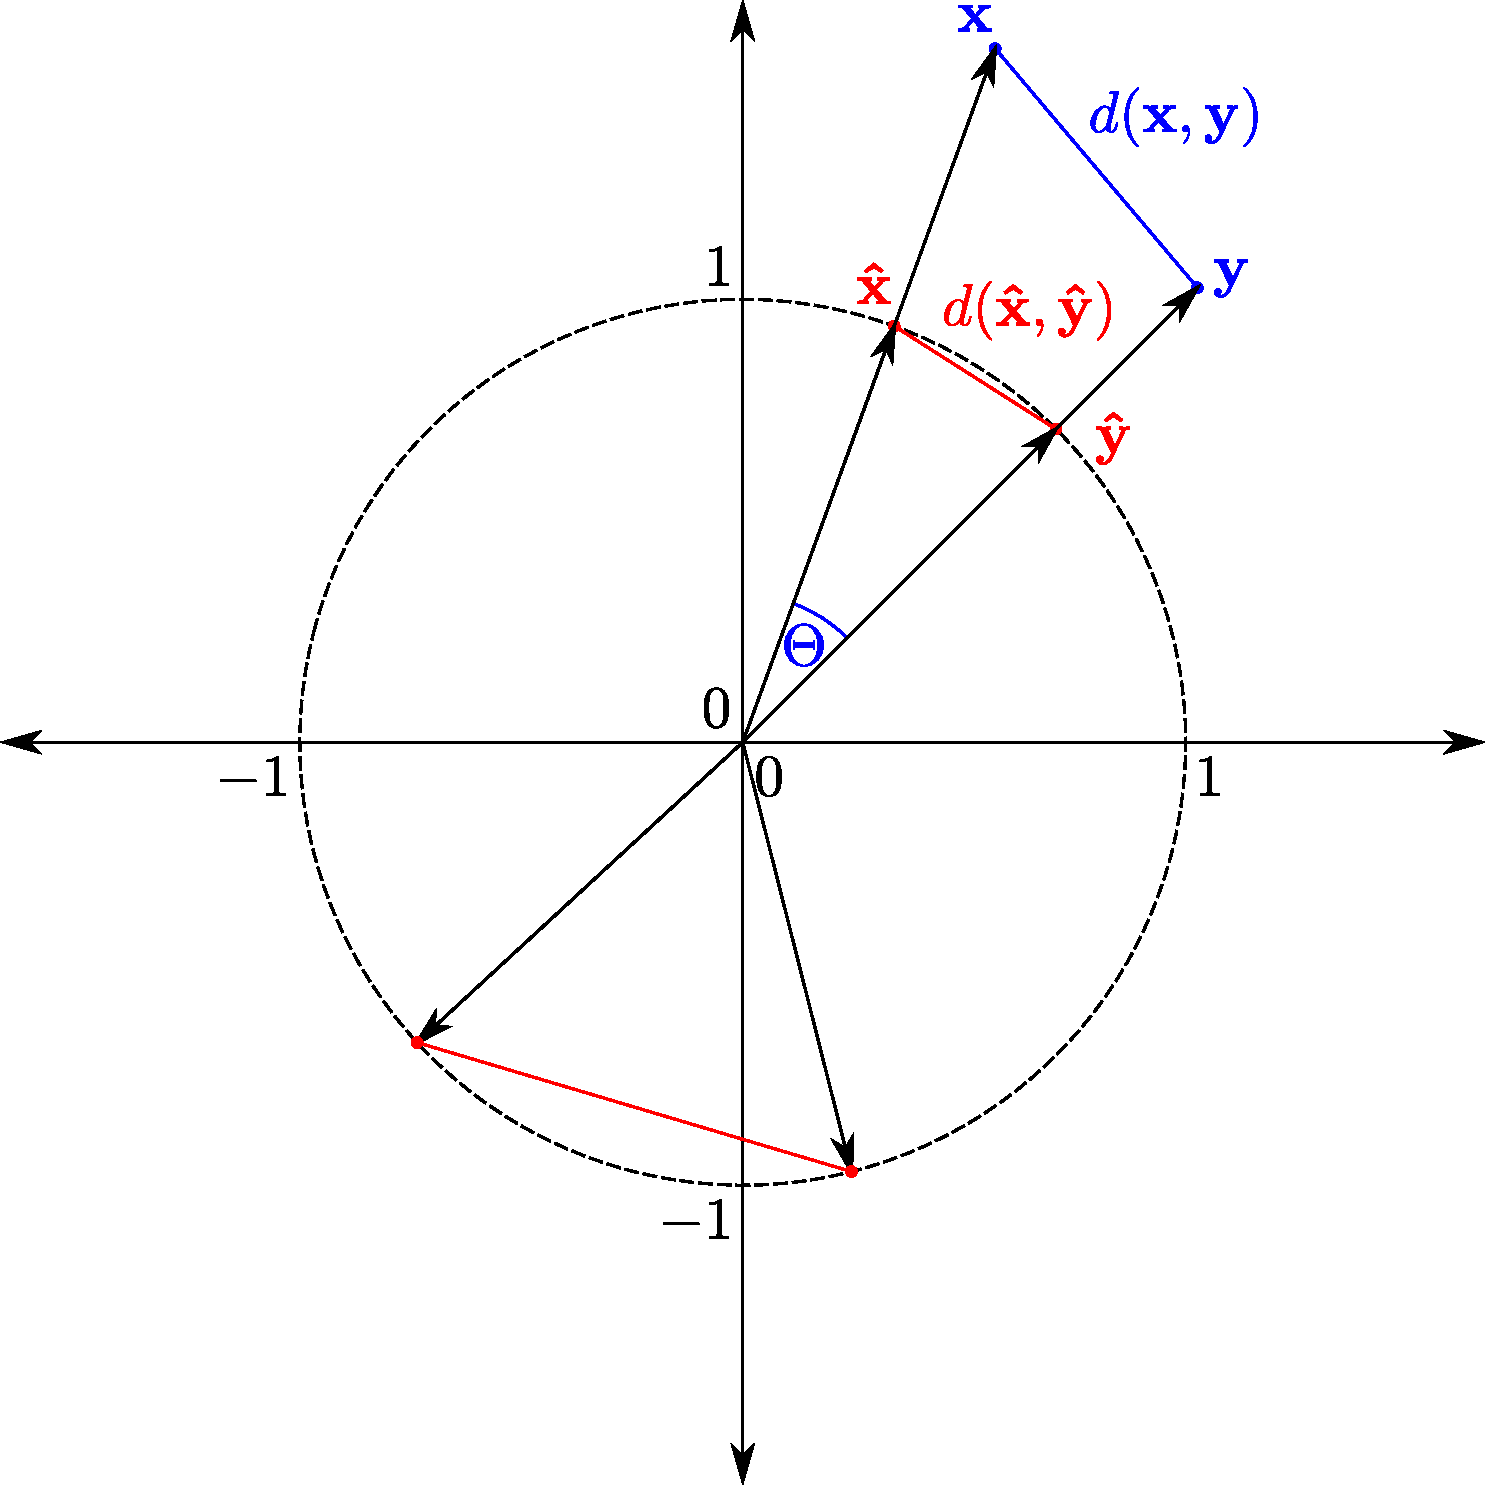
\includegraphics[width=\dimexpr\textwidth-2\fboxsep-2\fboxrule,fbox]{Graphics/L2_Euclidean.pdf}
    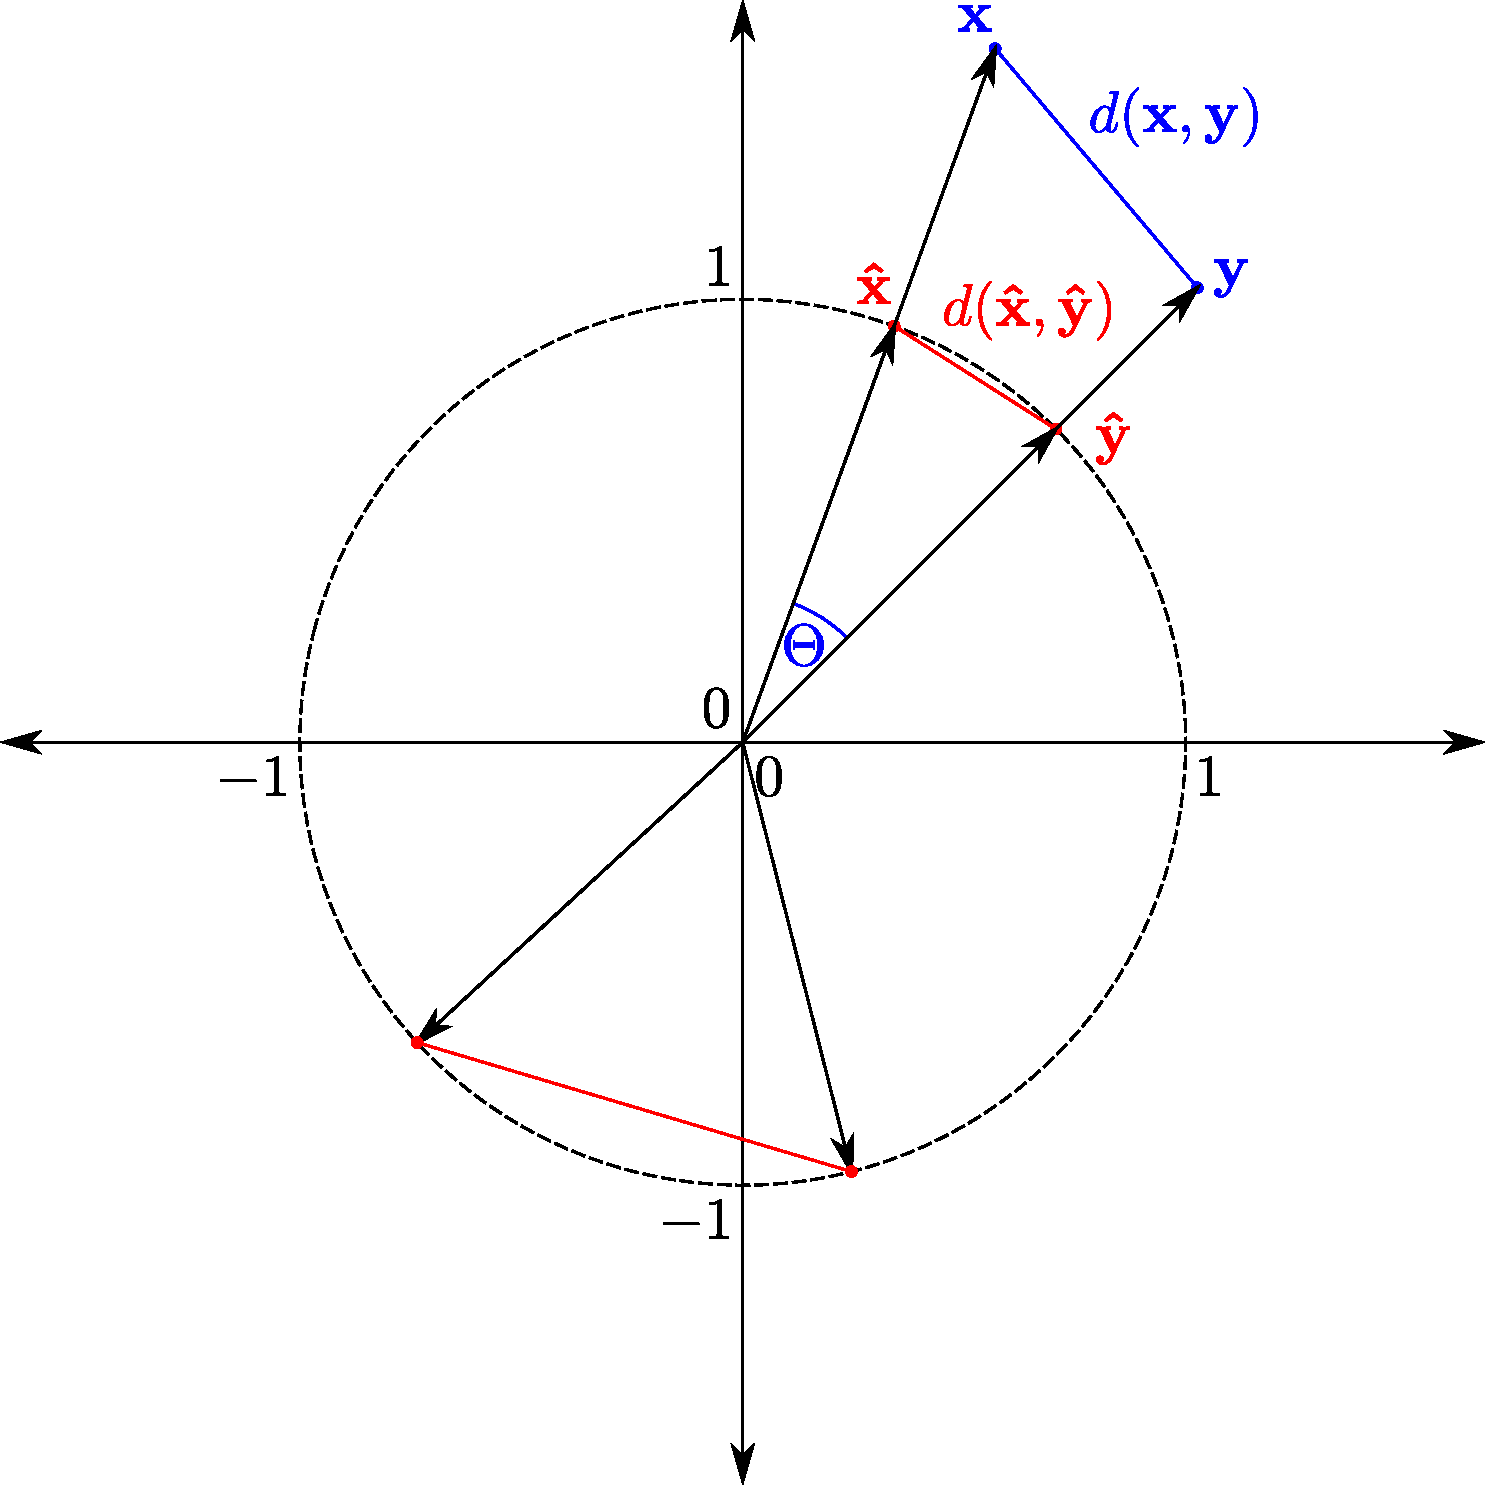
\includegraphics[width=\textwidth]{Graphics/L2_Euclidean.pdf}
    \caption[Graphical Background of L2 Normalisation]{\textbf{Graphical Background of L2 Normalisation.} blabla euclidean norm sphere.}
    \label{fig:L2_Normalisation_Background}
\end{figure}

\begin{empheq}{alignat = -1}
    \mathbf{\hat{x}}_i &= \frac{\mathbf{x}_i}{\Vert\mathbf{x}_i\Vert_2} \label{eq:l2_norm}
\end{empheq}

\begin{empheq}{alignat = -1}
    \Vert\mathbf{\hat{x}}_i\Vert_2 &= 1\label{eq:l2_result}
\end{empheq}

Chord distance $d_{\text{chord}}$ can be calculated when having two vectors, here as an exmaple named as $\mathbf{x}'$ and $\mathbf{y}'$ with the same L2-norm equal to a radius $r'$ of a sphere  centered to the origin of the coordinate system and an angle of $\Theta'$ (\autoref{eq:chord} and \autoref{fig:L2_Normalisation_Background}). The euclidean distance $d_{\text{eucl}}$ is equal to the chord distance for the same vectors $\mathbf{x}'$ and $\mathbf{y}'$ with L2-norm of $r'$.

\begin{empheq}{alignat = -1}
    &\Vert\mathbf{x}'\Vert_2 = \Vert\mathbf{y}'\Vert_2 = r' &&\to d_{\text{chord}}(\mathbf{x}',\mathbf{y}') &&= 2 \cdot r' \sin \left(\frac{\Theta'}{2}\right) \label{eq:chord}\\
    &&&&&= 2 \cdot \frac{d_{\text{eucl}}(\mathbf{x}',\mathbf{y}')}{2}\\
    &&&&&= d_{\text{eucl}}(\mathbf{x}',\mathbf{y}')\\
    &&&&&= \Vert\mathbf{x}' - \mathbf{y}'\Vert_2
\end{empheq}

Thus in this project chord distance can be calculated with the euclidean distance metric, posterior to the normalization with the L2-norm, which scales the vectors to the unit sphere (\autoref{eq:chord_eucl_1} to \autoref{eq:chord_eucl_2} and \autoref{fig:L2_Normalisation_Background}).

\begin{empheq}{alignat = -1}
    &\Vert\mathbf{\hat{x}}\Vert_2 = \Vert\mathbf{\hat{y}}\Vert_2 = 1 &&\to d_{\text{chord}}(\mathbf{\hat{x}},\mathbf{\hat{y}}) &&= d_{\text{eucl}}(\mathbf{\hat{x}},\mathbf{\hat{y}})\label{eq:chord_eucl_1}\\
    &&&&&= \Vert\mathbf{\hat{x}} - \mathbf{\hat{y}}\Vert_2 \label{eq:chord_eucl_2}
\end{empheq}

The used chord distance is proportional with the initially intended to use cosine distance as shown in \autoref{eq:chord_cos_1} to \autoref{eq:chord_cos_7}. Dividing the squared chord distance by 2 results in the cosinus distance of the vectors.

\begin{empheq}{alignat = -1}    
    &\Vert\mathbf{\hat{x}}\Vert_2 = \Vert\mathbf{\hat{y}}\Vert_2 = 1 &&\to d_{\text{chord}}(\mathbf{\hat{x}},\mathbf{\hat{y}})^2 &&= \Vert\mathbf{\hat{x}} - \mathbf{\hat{y}}\Vert_2^2\label{eq:chord_cos_1}\\
    &&&&&= (\mathbf{\hat{x}} - \mathbf{\hat{y}})^\top (\mathbf{\hat{x}} - \mathbf{\hat{y}})\label{eq:chord_cos_2}\\
    &&&&&= \mathbf{\hat{x}}^\top \mathbf{\hat{x}} - 2 \mathbf{\hat{x}}^\top \mathbf{\hat{y}} + \mathbf{\hat{y}}^\top \mathbf{\hat{y}}\label{eq:chord_cos_3}\\
    &&&&&= 2 - 2\mathbf{\hat{x}}^\top \mathbf{\hat{y}}\label{eq:chord_cos_4}\\
    &&&&&= 2 - 2 \cos(\Theta)\label{eq:chord_cos_5}\\
    &&&&&= 2 \cdot (1 - \cos(\Theta))\label{eq:chord_cos_6}\\
    &&&&&= 2 \cdot d_{\text{cos}}(\mathbf{x},\mathbf{y})\label{eq:chord_cos_7}
\end{empheq}

 Approximation of cosine distance by normalization with L2-norm followed by euclidean distance calculation is thus a possible and in this project used workaround to overcome the impossibility to use cosine distance.